\section{Atmoverb}

Si conclude infine con la progettazione del riverbero \emph{Atmoverb},
utilizzando le conoscenze maturate finora.

Il riverbero, come detto in precedenza, ha parametri di controllo relativi alle
condizioni atmosferiche dello spazio circostante all'ascoltatore. %\todo{Circostante a cosa?}
Gli algoritmi di base utilizzati saranno i medesimi implementati in precedenza:
\emph{Comb} con \emph{Low-Pass} (figura \ref{fig:amcombfir}) e
\emph{All-Pass lattice} (figura \ref{fig:amapfo})

I parametri di controllo Temperatura, Pressione, Gas

\lstinputlisting{Code/velsuono.dsp}


% \todo{mancano i commenti e manca un process che faccia capire a cosa serve il
%       codice. il senso di avere i blocchi separati viene meno se non funzionano
%       autonomi e se non ci sono i commenti}

Viene così definita la velocità del suono che in seguto influenza i tempi di
Delay dei vari Comb, in base alla posizione del suono nello spazio.

\begin{code}
//Posizione

xpos = hslider("[06]x[unit:]",50,0,100,1)/100;
ypos = hslider("[07]y[unit:]",50,0,100,1)/100;
zpos = hslider("[08]z[unit:]",10,0,100,1)/100;
\end{code}

Le variabili xpos, ypos, zpos servono per identidficare il punto di origine dell'evento sonoro;
Larghezza, lunghezza e altezza definiscono le dimensioni dello spazio riverberante.

\begin{code}
larghezza = hslider("[03]Larghezza[unit:mt]", 10,1,100,1);
lunghezza = hslider("[04]Lunghezza[unit:mt]", 10,1,100,1);
altezza = hslider("[05]Altezza[unit:mt]", 10,1,100,1);
\end{code}


I coefficenti di assorbimento delle pareti sono stati inseriti anch'essi, in quanto sappiamo
avere una certa influenza sul risultato sonoro. I valori sono compresi tra 0
(completamente assorbente) e 1 (completamente riverberante). I valori sono stati decisi
arbitrariamente per simulare una sala da concerto (il pavimento è il valore più basso per
l'influenza delle sedute).

\begin{code}
//Assorbimento Pareti

rifLat = .8;
rifFro = .5;
rifSoff = .85;
rifPav = .3;
\end{code}

Dato che il riverbero utilizza un'architettura Comb-AllPass, avente quindi diversi valori di g e di t
per i vari comb, calcoliamo i coefficenti utilizzando le variabili descritte prima.

\bigskip

Tempi:

\lstinputlisting{Code/combtimes.dsp}

Gain:

\lstinputlisting{Code/combg.dsp}

\pagebreak

Il risultato finale è poi inserito in una matrice mid/side, per sommare le componenti spaziali
e decodificato in seguito left/right per poterlo ascoltare in fase di test.

\lstinputlisting{Code/atmoverbprocess.dsp}


\begin{figure}[htp]
\centering
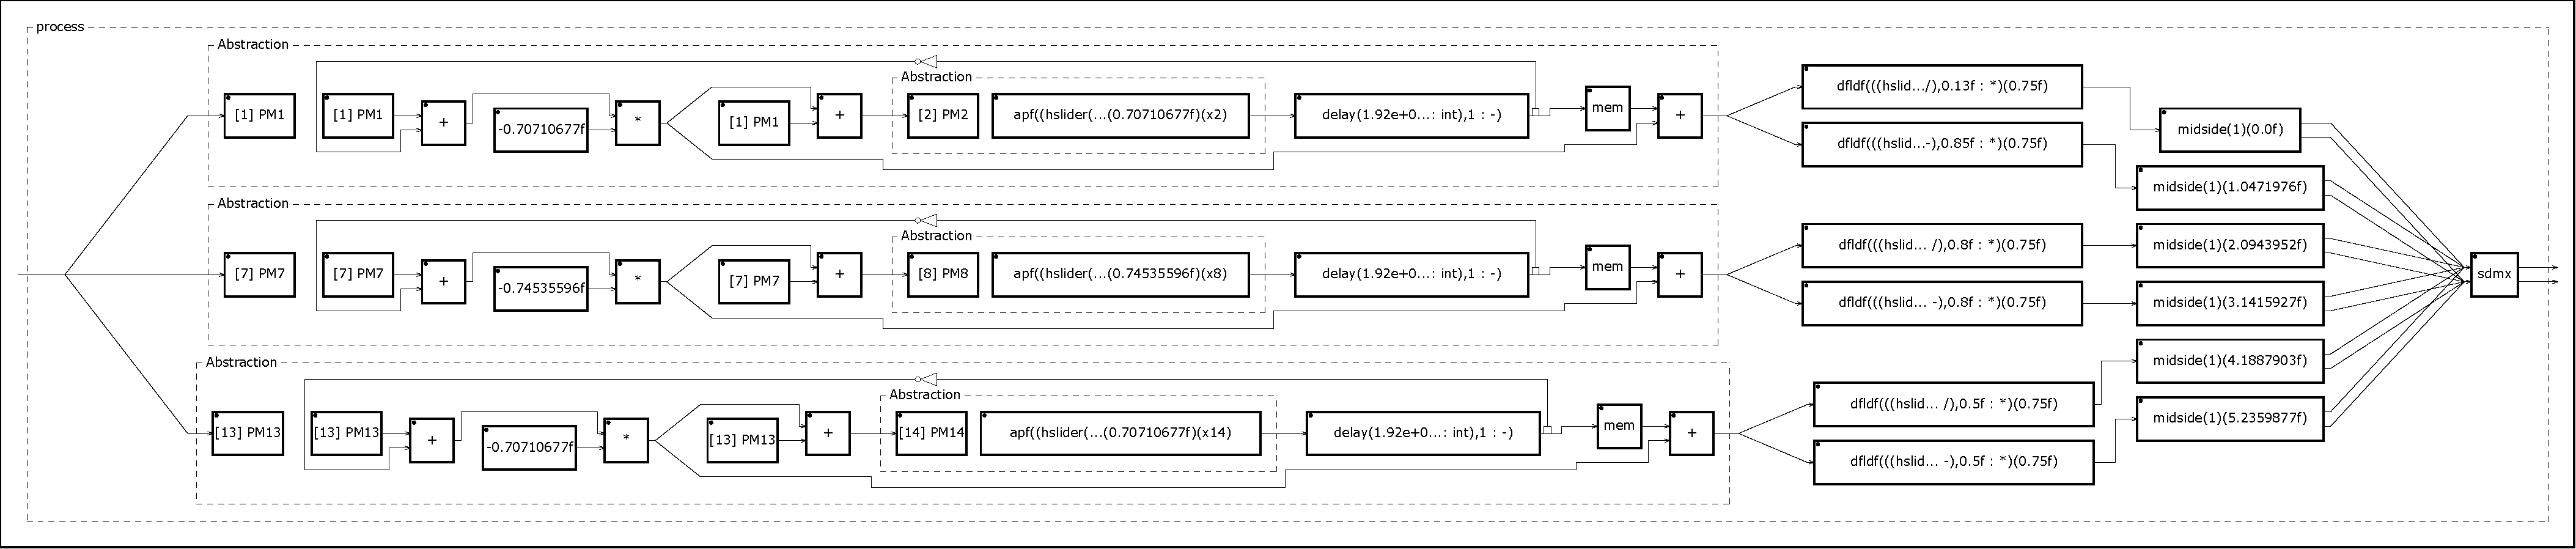
\includegraphics[width=1\textwidth]{Code/atmoverb-svg/process.pdf}
\label{fig:atmoverb}
\end{figure}
